\chapter{System Architecture}
\label{chap:System Architecture}

The main goal of this paper is to create a service that can convert single data-points into a continuous data-layer by interpolating missing data-points with the help of a machine learning approach. This service can then be used as a building block for other research-related activities/services, in order to abstract the complexity of the data-layer away while providing a good data quality.
In the context of temperature interpolation, we deal with three different architectural layers that are shown in Figure \ref{fig:system-architecture-overview}, and expose the service via a publish-subscribe pattern to other services \cite{bornholdt2019sane}.

\begin{figure}[h]
    \centering
    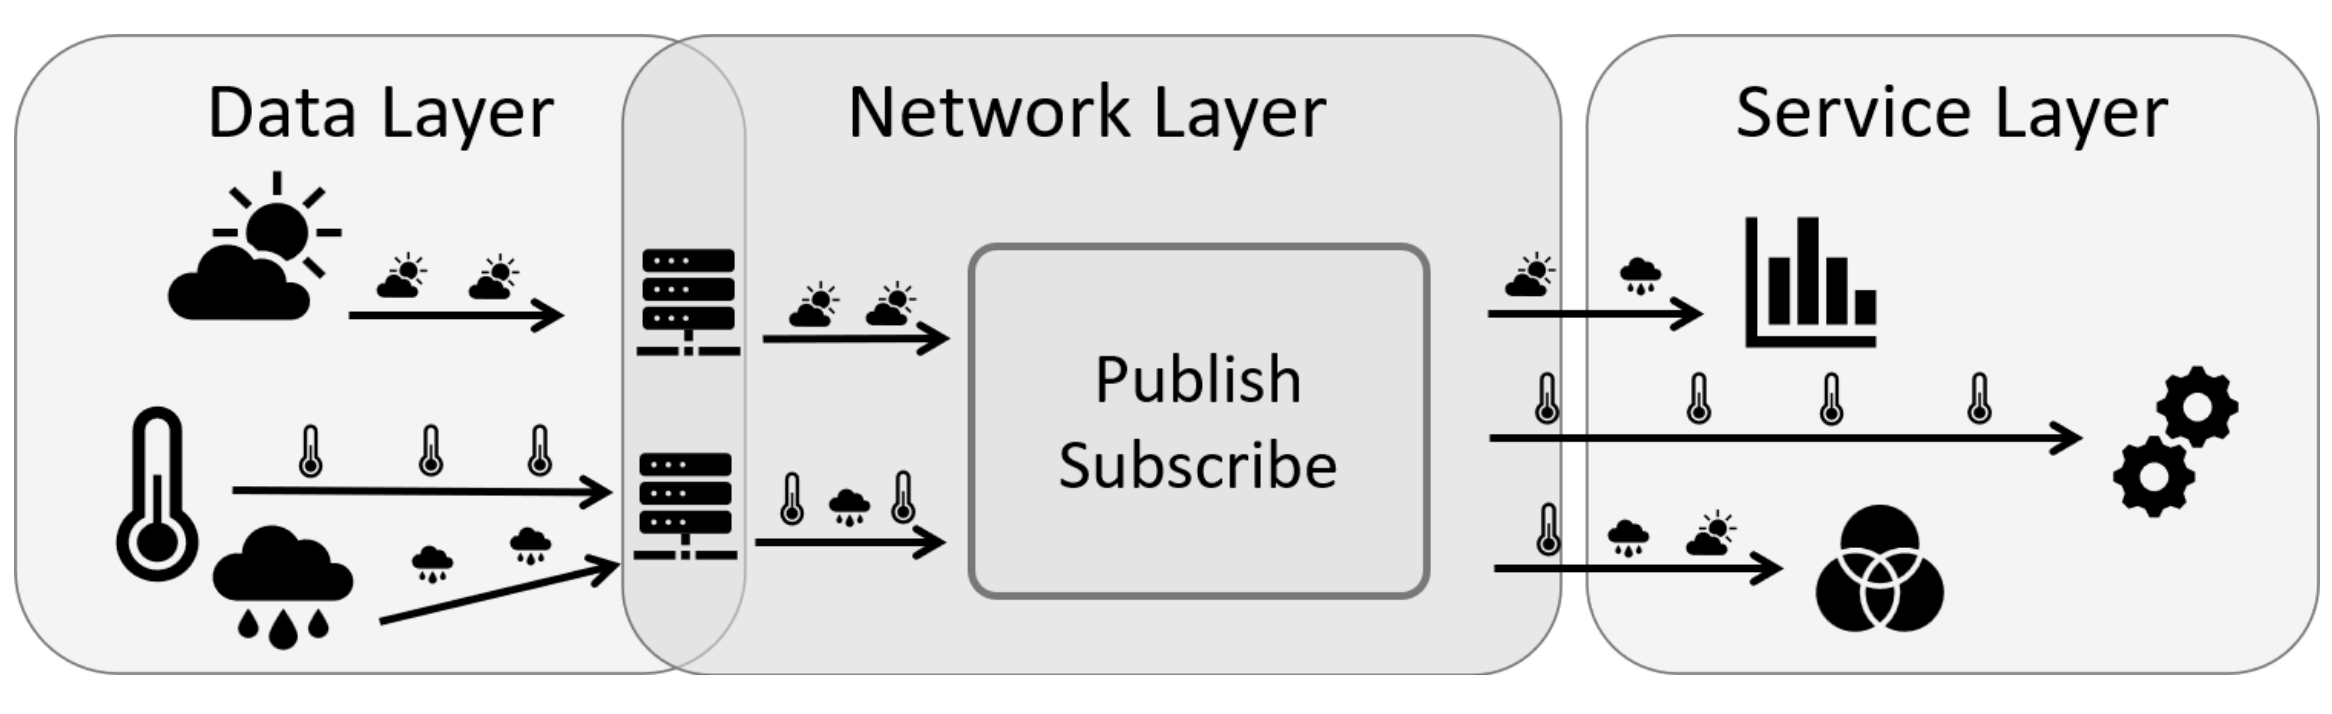
\includegraphics[width=\textwidth]{images/expose-system-architecture.png}
    \caption{In the data layer (left), a wide variety of environmental data is collected with the help of multiple sensors. These are connected to their citizen-owned local base stations, which manage access rights and forward collected data to subscribed services (right) via the decentralized publish-subscribe in the network layer (center).}
    \label{fig:system-architecture-overview}
\end{figure}

The \textit{data layer} consists of many different data sources. In the context of temperature sensing and prediction, this could include single (inexpensive) sensors such as the popular BMP280 \footnote{https://www.bosch-sensortec.com/products/environmental-sensors/pressure-sensors/bmp280/}, private weather stations such as sold by Netatmo \footnote{https://www.netatmo.com/en-gb/weather/weatherstation} hidden behind an API \footnote{https://dev.netatmo.com/apidocumentation/general}, public weather station data such as from the Deutscher Wetterdienst (DWD) \footnote{https://www.dwd.de/} which offer an API and historic weather data, or other geologically relevant data such as zoning plans which, in the case of the city of Hamburg in Germany, can be accessed via an OpenData platform provided by the State Office for Geoinformation and Surveying Hamburg \footnote{https://geoportal-hamburg.de/geo-online/}. In order to gain detailed insights into urban microclimates, we need fine-grained spatial and temporal data. As managing and maintaining such a large sensor network as a single entity can be quite challenging and cost intensive \cite{chapman2015birmingham}, we rely primarily on crowdsourced sensor data, in this case climate-related, from citizens, that give access to their personal sensors that they f.e. installed at home. This approach has been shown to work well in the densely populated urban area of Berlin, Germany \cite{meier2017crowdsourcing}, with the main challenge being data quality assessment due to faulty data from either broken, wrongly configured or wrongly installed sensors. The different data sources provide data streams which are then ingested by our interpolation service. Main challenges are the uncertainty in networks, such as single sensors or APIs not being available due to network interruptions, and the integration of many heterogeneous data sources that can contain data in different formats, time intervals or units of measurement etc.\\
The \textit{network layer} is responsible for integrating these different data sources in a consistent and reliable way and making them available for other services. The different sensors present in the data layer might have different vendors and programming interfaces, be located behind (vendor specific) APIs or are unreliably accessible due to unstable networks in edge environments. The network layer can be designed as a peer-to-peer (P2P) network based on the SkipNet approach \cite{harvey2002skipnet}, that utilizes the lookup efficiency of distributed hash tables and adds support for value-based range queries based on prefixes and attribute-value pairs. Another challenge in the context of the network layer, especially in the context of this paper, is also the integration of mobile sensors, which might not be constantly connected to a network while moving.\\
The data layer is then exposed via a publish-subscribe architecture \cite{bornholdt2019sane} to the \textit{service layer}, that offers subscriptions to and consumption of data streams and houses services such as our temperature interpolation service. These services can also build upon one another. An example for such a dependency could be a UHI detection service that relies on the temperature interpolation service and offers real-time detection of UHIs, which could trigger notifications/warnings for citizens living in the specific area.